%
% k3.tex
%
% (c) 2026 Prof Dr Andreas Müller
%
\begin{figure}
\centering
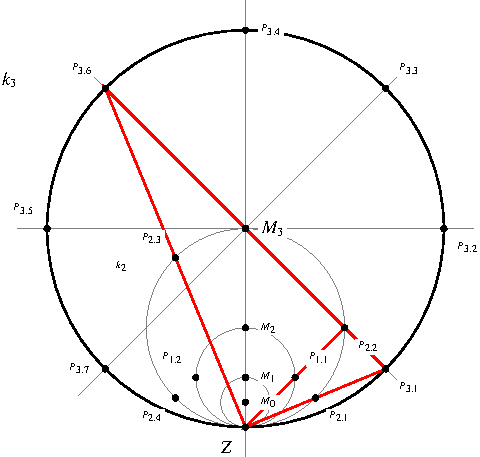
\includegraphics{papers/basel/images/k3.pdf}
\caption{Dritter Konstruktionsschritt: Kreis $k_3$ mit acht
äquidistanten Punkten.}
\end{figure}
